\documentclass[tikz,border=2pt]{standalone}
\usetikzlibrary{positioning,fit,backgrounds}
\begin{document}
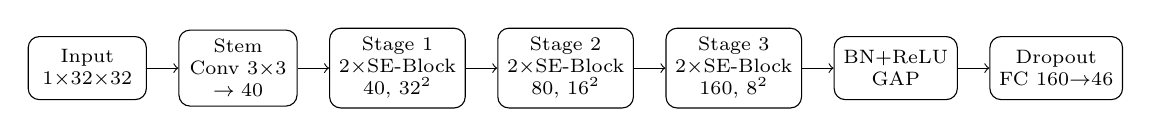
\begin{tikzpicture}[node distance=4mm,
  blk/.style={draw,rounded corners,minimum height=8mm,minimum width=15mm,font=\scriptsize,align=center}]
  \node[blk] (in)  {Input\\$1{\times}32{\times}32$};
  \node[blk,right=of in]  (stem) {Stem\\Conv $3{\times}3$\\$\to 40$};
  \node[blk,right=of stem] (s1) {Stage 1\\$2{\times}$SE-Block\\$40$, $32^2$};
  \node[blk,right=of s1]   (s2) {Stage 2\\$2{\times}$SE-Block\\$80$, $16^2$};
  \node[blk,right=of s2]   (s3) {Stage 3\\$2{\times}$SE-Block\\$160$, $8^2$};
  \node[blk,right=of s3]   (gap){BN+ReLU\\GAP};
  \node[blk,right=of gap]  (fc) {Dropout\\FC $160{\to}46$};
  \foreach \a/\b in {in/stem,stem/s1,s1/s2,s2/s3,s3/gap,gap/fc}
    \draw[->] (\a) -- (\b);
\end{tikzpicture}
\end{document}
